%================================================
% CAPÍTULO PONTEIROS
%================================================

\chapterimage{chapter_pointers.jpg} % Chapter heading image

\chapter{Ponteiros}

\section{Armazenamento Primário}\index{Armazenamento Primário}

Em um computador atual (2014), existem três tipos principais de armazenamento primário: \textbf{registradores do processador}; \textbf{cache do processador}, e; \textbf{memória principal}.

Registradores são pequenos locais de armazenamento, com tamanho estático, contidos no processador. Por fazerem parte do \textit{ISA (Instruction Set Architecture)}, variam com a arquitetura (x86, x86\_64, MIPS etc). Um exemplo de registradores de uso geral da arquitetura x86\_64 é: \textit{rax, rbx, rcx, rdx}.

A cache do processador é um contêiner de dados intermediário e de acesso aleatório com maior capacidade que os registradores. Ela se situa entre a memória principal e o próprio processador com o intuito de diminuir o tempo médio de acesso às informações; podendo ser subdividida em cache de instruções (lida apenas com a leitura da memória), cache de dados (trata da leitura e escrita da memória) e \textit{TLB - Translation lookaside buffer} (com a finalidade de agilizar a tradução da memória virtual x física).

O termo ``Memória Principal'' é comumente usado como referência à memória RAM \textit{(Random Access Memory)}, uma vez que nesta reside a grande porção de dados utilizados antes e/ou após o processamento. Essa referência se dá, também, pela transparência que os registradores e a cache do processador tem em comparação à memória principal, tendo em vista a utilizaçao direta dos dados contidos nela quando no desenvolvimento de software.

Há alguns detalhes importantes a serem ressaltados a respeito desses três repositórios primários de dados.

\begin{enumerate}
\item A memória principal (RAM), distintamente dos registradores e da cache, não se encontra no processador mas sim conectada a ele através do barramento de memória que, por sua vez, subdivide-se em dois: barramento de endereço e barramento de dados [\autoref{fig:memory_controller}].
\item O gerenciamento da memória cache, mesmo que possível através de instruções como INVD e WBINVD na arquitetura x86, é e deve, por segurança, ser deixado ao encargo do próprio processador, salvo casos realmente justificáveis.
\item Os dados de todos eles são obtidos por endereçamento, ou seja, por indexação, mas o que os torna diferentes, à visão do programador, é o fato de os registradores e a cache só serem acessados dessa forma pelo microcódigo da arquitetura, enquanto a memória principal pode o ser por endereçamento via código de máquina (programa residente na própria memória).
\end{enumerate}

% \clearpage
\begin{figure}[!htp]
  \centering
  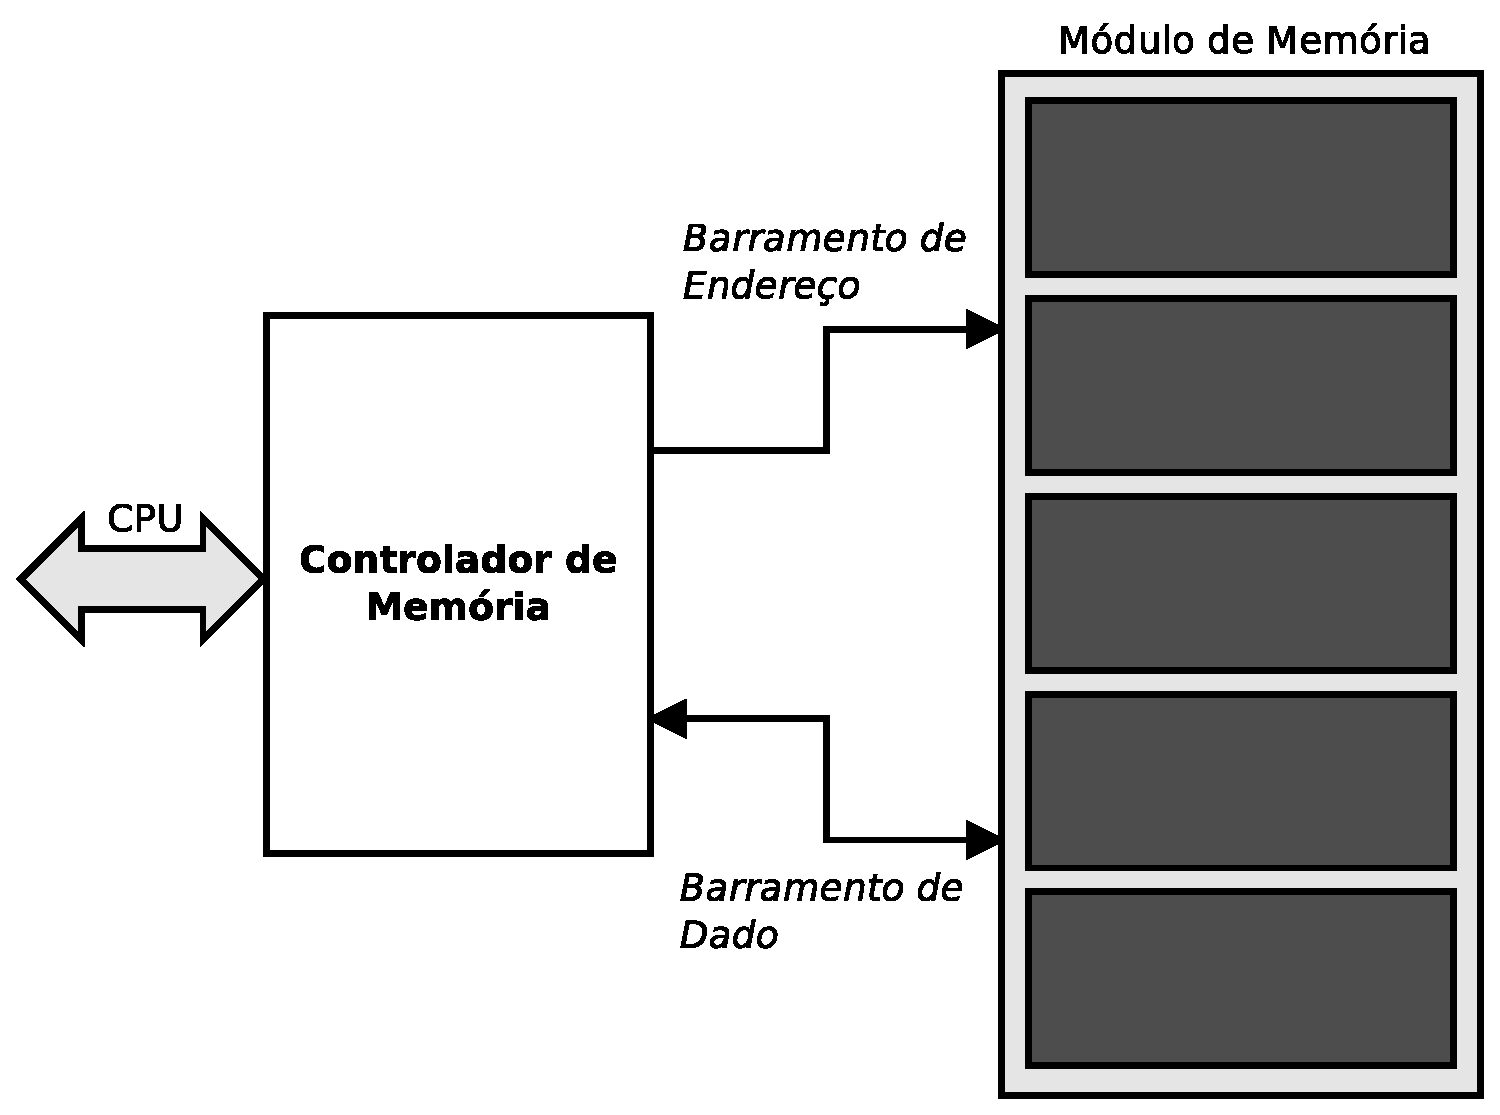
\includegraphics[scale=0.5, keepaspectratio=true]{memory_controller.eps}
  \caption{Barramentos de Endereço e de Dados}
 \label{fig:memory_controller}
\end{figure}

%------------------------------------------------

\subsection{Memória Principal}\index{Armazenamento Primário!Memória Principal}

Sobre a memória principal.

%================================================

\section{Usando Ponteiros}\index{Usando Ponteiros}

Como usar ponteiros.

%================================================

\section{Usando Vetores}\index{Usando Vetores}

Como usar vetores.

%================================================

\section{Vetores NÃO são Ponteiros}\index{Vetores NÃO são Ponteiros}

Vetores não são ponteiros.